% OpenMP для разных стратегий распараллеливания для Римановского решателя.
\subsection{Сравнение стратегий распараллеливания с помощью OpenMP для микропроцессора Intel Xeon Phi KNL}

Микропроцессоры Intel Xeon Phi KNL 7290, для которых проводилось исследование по распараллеливанию, содержат по 72 ядра, в каждом из которых возможно запустить  по 4 потока, что дает суммарно 288 потоков для одного процессора.
Ввиду этого применение распараллеливания с помощью OpenMP является ожидаемым, так как способно существенно ускорить исполняемый код.
Были проанализированы 3 стратегии распараллеливания (см. рис.~\ref{fig:text_3_omp1_modes}), описание которых приведено ниже.

\begin{figure}[ht]
\centering
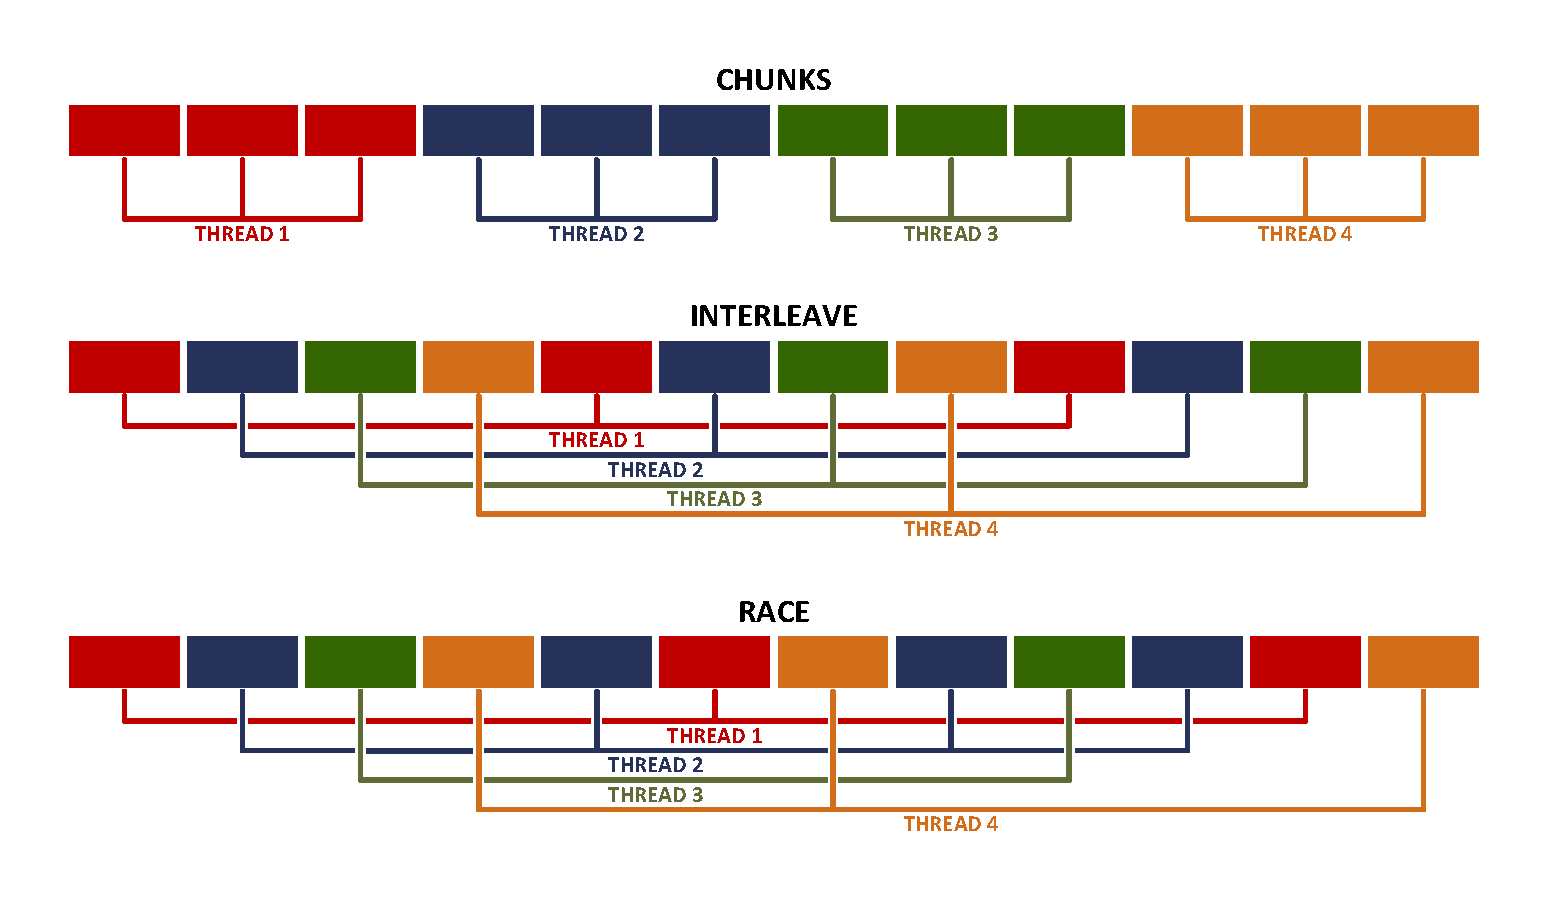
\includegraphics[width=0.8\textwidth]{./pics/text_3_omp1/modes.pdf}
\singlespacing
\captionstyle{center}\caption{Иллюстрация работы трех рассматриваемых стратегий распараллеливания вычислений: CHUNKS, INTERLEAVE, RACE.}
\label{fig:text_3_omp1_modes}
\end{figure}

В качестве первой стратегии распараллеливания была использована стратегия CHUNKS, в которой массивы входных данных были разделены на равные непрерывные части по числу используемых потоков, каждый поток обрабатывал свои участки массивов входных данных (на листинге~\ref{lst:text_3_strat_chunks} \texttt{nt} -- общее количество потоков, \texttt{solver\_16} -- указатель на решатель для обработки 16 экземпляров задачи Римана).

\begin{singlespace}
\begin{lstlisting}[caption={Распараллеливание римановского решателя с помощью стратегии CHUNKS.},label={lst:text_3_strat_chunks}]
#pragma omp parallel
{
    int tn = omp_get_thread_num();
    int lb = (int)((c/FP16_VECTOR_SIZE)*((double)tn/(double)nt));
    int ub = (int)((c/FP16_VECTOR_SIZE)*((double)(tn + 1)/(double)nt));

    for (int i = lb * FP16_VECTOR_SIZE;
         i < ub * FP16_VECTOR_SIZE;
         i += FP16_VECTOR_SIZE)
    {
        solver_16(dl + i, ul + i, vl + i, wl + i, pl + i,
                  dr + i, ur + i, vr + i, wr + i, pr + i,
                  d + i, u + i, v + i, w + i, p + i);
    }
}
\end{lstlisting}
\end{singlespace}

Во второй стратегии -- INTERLEAVE -- массивы входных данных были разделены на участки по 16 элементов и распределялись между потоками в шахматном порядке (на листинге~\ref{lst:text_3_strat_interleave} \texttt{c\_base} -- длина массивов входных данных без учета эпилога цикла, \texttt{nt} и \texttt{solver\_16} имеют тот же смысл, что и на листинге~\ref{lst:text_3_strat_chunks}).

\begin{singlespace}
\begin{lstlisting}[caption={Распараллеливание римановского решателя с помощью стратегии INTERLEAVE.},label={lst:text_3_strat_interleave}]
#pragma omp parallel
{
    int tn = omp_get_thread_num();

    for (int i = tn * FP16_VECTOR_SIZE;
         i < c_base;
         i += nt * FP16_VECTOR_SIZE)
    {
        solver_16(dl + i, ul + i, vl + i, wl + i, pl + i,
                  dr + i, ur + i, vr + i, wr + i, pr + i,
                  d + i, u + i, v + i, w + i, p + i);
    }
}
\end{lstlisting}
\end{singlespace}

Третья стратегия -- RACE -- основана на ведении глобального адреса следующего готового к обработке участка входных данных.
Как только очередной поток освобождается, он приступает к обработке следующих свободных 16 экземпляров задачи.
Таким образом была предпринята попытка избавиться от простоев потоков в случае разного времени выполнения отдельных экземпляров задачи.

\begin{singlespace}
\begin{lstlisting}[caption={Распараллеливание римановского решателя с помощью стратегии RACE.},label={lst:text_3_strat_race}]
int g = 0;
#pragma omp parallel
{
    int i = 0;
    bool is_break = false;

    while (true)
    {
        #pragma omp critical
        {
            if (g >= c_base)
            {
                is_break = true;
            }
            else
            {
                i = g;
                g += FP16_VECTOR_SIZE;
            }
        }

        if (is_break)
        {
            break;
        }

        solver_16(dl + i, ul + i, vl + i, wl + i, pl + i,
                  dr + i, ur + i, vr + i, wr + i, pr + i,
                  d + i, u + i, v + i, w + i, p + i);
    }
} 
\end{lstlisting}
\end{singlespace}

На листинге~\ref{lst:text_3_strat_race} \texttt{g} -- глобальный счетчик следующей свободной партии экземпляров задачи Римана, доступный всем потокам.
Для его проверки и продвижения требуется блокировка.
Для всех описанных стратегий были выполнены тестовые расчеты на суперкомпьютере МВС-10П.

Единственным параметров теста является максимальное количество потоков, на которых нужно выполнять прогон.
При этом сначала тесты прогоняются на невекторизованном решателе с использованием одного потока (относительно этого запуска считается суммарное ускорение решателя).

После этого выполняется запуск векторизованного решателя для различного количества потоков, начиная от 1 и заканчивая 288.
По результатам прогона выдается время работы как невекторизованного решателя на одном потоке, так и векторизованной версии для разного количества потоков.
Отдельно выполнялись прогоны для стратегий распараллеливания CHUNKS, INTERELEAVE и RACE.
По результатам прогонов были построены графики суммарного ускорения векторизованного и распараллеленного римановского решателя для всех трех стратегий, данные графики представлены на рис.~\ref{fig:text_3_omp1_main_graph}.

\begin{figure}[ht]
\centering
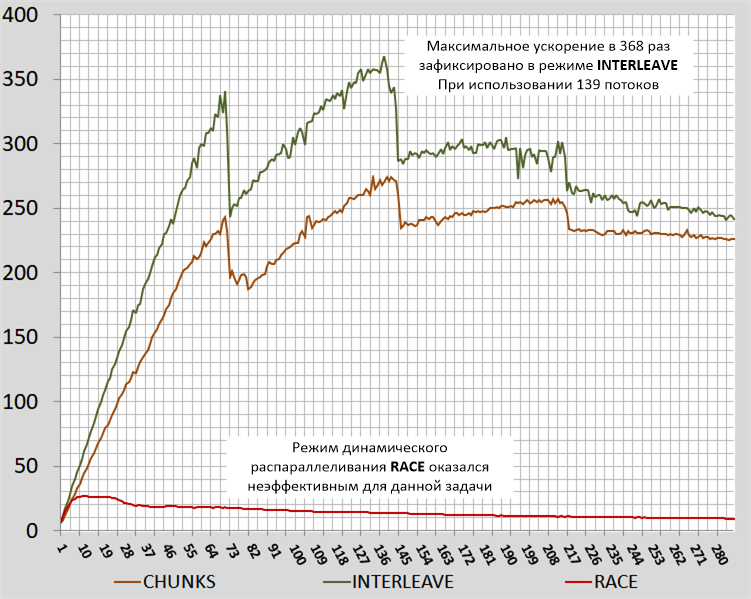
\includegraphics[width=1.0\textwidth]{./pics/text_3_omp1/main_graph.png}
\singlespacing
\captionstyle{center}\caption{График ускорения и эффективности распараллеливания векторизованного римановского решателя на микропроцессоре Intel Xeon Phi KNL.}
\label{fig:text_3_omp1_main_graph}
\end{figure}

Из рис.~\ref{fig:text_3_omp1_main_graph} видно, что стратегия распараллеливания RACE является нежизнеспособной даже на сравнительно небольшом числе потоков.
Блокировка глобального ресурса (счетчик следующей свободной партии задач), оказывается фатальной и приводит к простою потоков.

Из двух других стратегий стратегия INTERLEAVE показала себя лучше, продемонстрировав максимальное ускорение более 50 раз на 139 потоках.

На графиках явно просматриваются 4 характерные участка, длина которых совпадает с количеством ядер микропроцессора Intel Xeon Phi KNL 7290 (72 ядра).
На первом участке масштабируемость распараллеливания близка к линейной.
На втором участке наблюдается сначала некоторое снижение эффективности, но затем при дальнейшем увеличении количества потоков удается добиться дополнительного ускорения.
На третьем и четвертом участках графиков наблюдается снижение производительности.
Это ожидаемо, так как каждое ядро микропроцессора содержит два векторных исполнительных устройства и при запуске на ядре трех или четырех потоков начинается конкуренция за данные исполнительные устройства.
